\documentclass[a4paper, 12pt]{article}

\usepackage[portuges]{babel}
\usepackage[utf8]{inputenc}
\usepackage{amsmath}
\usepackage{indentfirst}
\usepackage{graphicx}
\usepackage[colorinlistoftodos]{todonotes}

\usepackage[pdftex]{hyperref}




\begin{document}
%\maketitle

\begin{titlepage}
	\begin{center}
		\huge{Universidade Federal de Ouro Preto}

\vspace{10pt}
\begin{figure}[!ht]
\centering

\includegraphics[width=4cm]{img/logo.jpg}
\end{figure}
        
        \vspace{85pt}
        
		\textbf{\LARGE{Engenharia de Software II}}\\
		\large{Sistema de \textit{Empréstimo de Jogos}\\ Grupo: \textit{cafeína++;}}
		\vspace{160pt}
		
	\end{center}
	
	\begin{flushleft}
		\begin{tabbing}
			Alunos:\qquad\qquad\= Caio Soares Costa \\
			\>Cibele Oliveira Ferreira \\
            \>Eduardo Matosinhos Florinda \\
            \>Gabriel Caetano Araújo \\
			Professor:\> Johnatan Oliveira \\
			Horário:\> Seg e Qua - 08:20 - 10:00\\
		
	\end{tabbing}
		  
	\end{flushleft}
	
	\begin{center}
		%\vspace{\fill}
		Ouro Preto, \today
	\end{center}
\end{titlepage}
%%%%%%%%%%%%%%%%%%%%%%%%%%%%%%%%%%%%%%%%%%%%%%%%%%%%%%%%%%%
\newpage
\tableofcontents
\thispagestyle{empty}

\newpage
\pagenumbering{arabic}

%%%%%%%%%%%%%%%%%%%%%%%%%%%%%%%%%%%%%%%%%%%%%%%%%%%%%%%%%
%%%%%%%%%%%%%%%%%%%%%%%%%%%%%%%%%%%%%%%%%%%%%%%%%%%%
\section{Histórico de Revisões}

\begin{table}[!h]
\centering
\begin{tabular}{|l|l|l|l|}
\hline
\multicolumn{1}{|c|}{Data} & \multicolumn{1}{c|}{Versão} & \multicolumn{1}{c|}{Descrição}                 & Autor       \\ \hline
10/03/2021                 & 0.0                         & Justificativa do processo de software          & Eduardo     \\ \hline
10/03/2021                 & 0.0                         & Levantamento de requisitos                     & Caio, Cibele e Gabriel            \\ \hline 
20/03/2021                 & 0.0                         & Especificação de requisitos                     & Caio, Cibele e Gabriel            \\ \hline
                           &                             &                                                &             \\ \hline 
\end{tabular}
\caption{Revisões do Documento}
\label{tab:my-table}
\end{table}

\section{Processo e Software}
% Apresente aqui uma breve explicação do modelo de processo de software escolhido. Lembre-se, vocês precisam citar claramente o modelo de processo de software escolhido, por exemplo, \textbf{SCRUM}.

A equipe ‘‘cafeína++;’’, desenvolvedora do software ‘‘Game Stonks’’, adotou o processo de desenvolvimento incremental. Esta escolha levou em consideração o fato deste modelo permitir obter feedback rápido do cliente a partir de pequenas entregas iterativas. Desta forma, o custo de acomodar mudanças nos requisitos e o risco de falha global do projeto é reduzido. Ademais, é possível validar o sistema parcial a cada incremento, sendo uma vantagem já que o cliente não precisa esperar a entrega final para usá-lo. Portanto, os serviços de mais alta prioridade são entregues primeiros.

\section{Cronograma}
% Vocês devem apresentar aqui o cronograma das atividades e seus respectivos responsáveis. 

\begin{table}[!h]
\centering
\begin{tabular}{|l|l|l|}
\hline
\multicolumn{1}{|c|}{Nome} & \multicolumn{1}{c|}{Tarefa}                                                                                   & \multicolumn{1}{c|}{Prazo} \\ \hline
Eduardo                    & Definir tema do projeto                                                                                       & 01/03  \\ \hline
Gabriel                    & Criar repositório no GitHub                                                                                   & 01/03  \\ \hline
Eduardo                    & \begin{tabular}[c]{@{}l@{}}Escolha e justificativa do Processo de \\ Desenvolvimento de Software\end{tabular} & 13/03  \\ \hline
Caio, Cibele e Gabriel     & Levantamento dos requisitos do software                                                                       & 13/03  \\ \hline
\begin{tabular}[c]{@{}l@{}}Caio, Cibele e\\ Gabriel \end{tabular}     & Especificação de requisitos                               & 20/03  \\ \hline
Gabriel                    & Definição da tecnologia, arquitetura e classes                                                                & 20/03  \\ \hline
\begin{tabular}[c]{@{}l@{}}Caio, Cibele, Eduardo e\\ Gabriel \end{tabular} & Definir backlog                                               & 24/03  \\ \hline

\end{tabular}
\caption{Cronograma}
\label{tab:my-table}
\end{table}

\section{Levantamento de Requisitos}
% Independente da metodologia de desenvolvimento utilizada, o levantamento de requisitos é o ponto de partida de qualquer projeto de software, pois é a partir dos resultados obtidos durante esta etapa que será possível definir como as próximas etapas do desenvolvimento serão executadas.

% Apresente a técnica que a sua equipe irá utilizar, explique porquê de tal técnica e quais os resultados obtidos.
\subsection{Diagrama de Caso de Uso}

\begin{figure}[ht!]
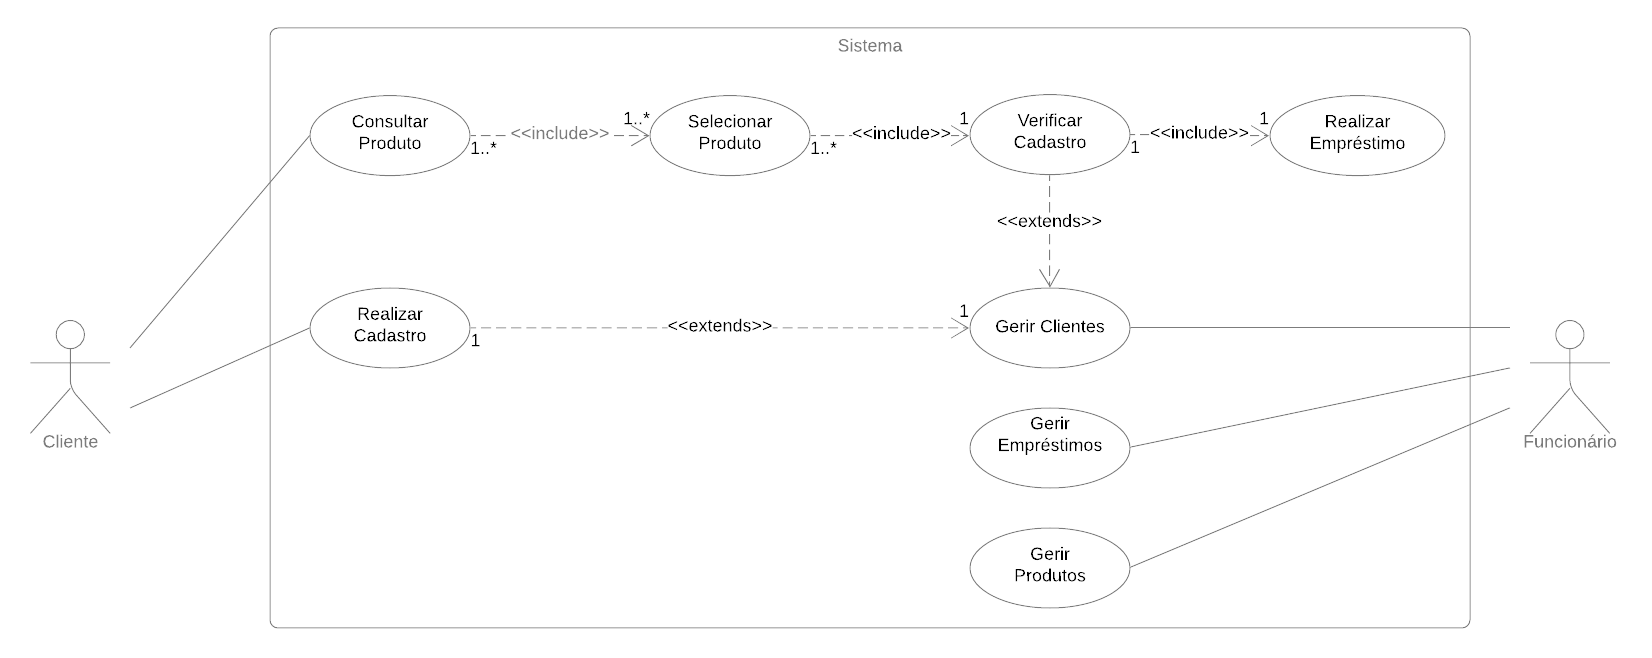
\includegraphics[width=\textwidth]{./img/casos-de-uso.png}
\centering
\caption{Diagrama de Casos de Uso}\label{img:casos-de-uso}
\end{figure}

\subsection{Descrição de Caso de Uso}

\begin{table}[!h]
\centering
\begin{tabular}{|l|l|l|}
\hline
\multicolumn{1}{|c|}{Código} & \multicolumn{1}{c|}{Serviço} & \multicolumn{1}{c|}{Descrição} \\ \hline
RF01  & Realizar cadastro   & \begin{tabular}[c]{@{}l@{}}Permite o cliente se cadastrar no sistema. \end{tabular} \\ \hline
RF02  & Consultar produtos  & \begin{tabular}[c]{@{}l@{}}Permite o cliente consultar um jogo no \\ sistema. \end{tabular} \\ \hline
RF03  & Selecionar produto  & \begin{tabular}[c]{@{}l@{}}Permite o cliente selecionar um jogo para \\ empréstimo. \end{tabular} \\ \hline
RF04  & Verificar cadastro  & \begin{tabular}[c]{@{}l@{}}Possibilita a verificação do cadastro do cliente \\ no sistema. \end{tabular}  \\ \hline
RF05  & Realizar empréstimo & \begin{tabular}[c]{@{}l@{}}Efetiva o empréstimo do produto para o cliente \\ que o selecionou.\end{tabular}  \\ \hline
RF06  & Gerir clientes      & \begin{tabular}[c]{@{}l@{}}Gerencia os clientes que estão cadastrados no \\ software. \end{tabular}  \\ \hline
RF07  & Gerir empréstimos   & \begin{tabular}[c]{@{}l@{}}Gerencia os empréstimos realizados.\end{tabular}  \\ \hline
RF08  & Gerir produtos      & \begin{tabular}[c]{@{}l@{}}Gerencia os produtos (jogos) do software. \end{tabular}  \\ \hline

\end{tabular}
\caption{Descrição de Casos de Uso}
\label{tab:descricao-casos-de-uso}
\end{table}

% \textit{Para o levantamento de requisitos, o analista dispõe de algumas técnicas que são utilizadas de acordo com o perfil do cliente. Existem diversas técnicas, cada uma adequada para um cenário específico, e dentre as comumente utilizadas podemos citar as seguintes técnicas:}

% \begin{enumerate}
% \item Descoberta de Requisitos  (Pontos de vista)
% \item Entrevistas
% \item Cenários
% \item Casos de Uso
% \item Etnografia 
% \end{enumerate}

\section{Especificação de Requisitos}
\subsection{Requisitos Funcionais}
\textbf{RF01--} \textbf{Realizar cadastro:} Este serviço realiza todas as tarefas relacionadas à autenticação.
\begin{itemize}
    \item \textbf{Criar login:} Campo de texto para login.
    \item \textbf{Criar senha:} Campo de texto para senha.
    \item \textbf{Recuperar senha:} Permite recuperar a senha.
    \item \textbf{Alterar senha:} Permite alterar a senha.
    \item \textbf{Autenticar login e senha:} Valida o login e senha.
    \item \textbf{Sair do sistema:} Realiza o logout.
\end{itemize}

\textbf{RF02--} \textbf{Consultar Produto:} Este serviço possibilita que o usuário consulte se o jogo que ele irá pegar emprestado está disponível.
\begin{itemize}
    \item \textbf{Filtrar Jogos:} Possibilita que o usuário filtre os jogos de acordo com tema, nome e empresa de desenvolvedora.
    \item \textbf{Consultar Disponibilidade:} Possibilita que o usuário veja se um jogo estará disponível para empréstimo.
\end{itemize}

\textbf{RF03--} \textbf{Selecionar Produto:} Este serviço permite ao usuário adicionar um jogo ao carrinho para o empréstimo.

\begin{itemize}
    \item \textbf{Adicionar Jogo:} Permite adicionar jogos ao carrinho.
    \item \textbf{Remover Jogos:} Permite remover jogos do carrinho.
    \item \textbf{Atualizar valor de jogos no carrinho:} Atualiza o valor total dos jogos para empréstimo.
\end{itemize}

\textbf{RF04--} \textbf{Verificar cadastro:} Este serviço faz a verificação do cadastro do usuário e validação das informações
\begin{itemize}
    \item \textbf{Autenticação de login:} Verifica se o usuário está cadastrado no sistema antes de prosseguir com o empréstimo.
    \item \textbf{Autenticação de informações:} Verifica se as informações inseridas pelo usuário estão corretas.
    \item \textbf{Verificar pendências:} Verifica se o usuário possui algum débito registrado no sistema.
\end{itemize}

\textbf{RF05--} \textbf{Realizar Empréstimos:} Este serviço possibilita que o usuário efetue o empréstimo do jogo que deseja.
\begin{itemize}
    \item \textbf{Validar dados do cartão:} Valida os dados de cartão de crédito do usuário.
    \item \textbf{Efetua pagamento:} Utiliza uma API para realizar o pagamento do empréstimo solicitado pelo usuário.
    \item \textbf{Libera Empréstimo:} Disponibiliza para o usuário os jogos que ele escolheu por empréstimo.
\end{itemize}

\textbf{RF06--} \textbf{Gerir clientes:} Este serviço realiza todas as tarefas relacionadas ao cadastro de usuários do sistema.
\begin{itemize}
    \item \textbf{Cadastrar usuário:} Permite cadastrar um usuário no sistema.
    \item \textbf{Consultar usuário:} Permite visualizar todos os dados de um usuário registrado.
    \item \textbf{Buscar usuário:} Permite fazer uma busca de um usuário no sistema.
    \item \textbf{Alterar dados do usuário:} Permite atualizar todos os dados relacionados a um usuário.
    \item \textbf{Remover usuário:} Permite excluir o usuário do sistema.
\end{itemize}

\textbf{RF07--} \textbf{Gerir empréstimos:} Este serviço realiza todas as tarefas relacionadas à contabilidade de gastos e lucros do Game Stonks.
\begin{itemize}
    \item \textbf{Consultar empréstimos:} Permite ao administrador visualizar os empréstimos realizados.
    \item \textbf{Consultar lucro por jogo:} Permite ao administrador visualizar lucro por empréstimos de jogos.
    \item \textbf{Consultar resumo financeiro:} Permite ao administrador visualizar o resumo financeiro.
    \item \textbf{Exportar resumo financeiro:} Exporta relatório em formato CSV.
    \item \textbf{Registrar gastos com compra de jogos:} Permite que o administrador adicione os gastos com a compra de jogos.
    \item \textbf{Registrar lucro por jogo:} Permite que o administrador adicione os lucros por empréstimos de jogos.
\end{itemize}

\textbf{RF08--} \textbf{Gerir produtos:} Este serviço realiza todas as tarefas relacionadas ao gerenciamento dos jogos.
\begin{itemize}
    \item \textbf{Registrar jogos:} Permite que o administrador adicione as informações pertinentes aos jogos.
    \item \textbf{Consultar jogos:} Permite ao administrador visualizar os jogos cadastrados no sistema.
    \item \textbf{Editar jogos:} Permite ao administrador editar as informações dos jogos cadastrados no sistema.
    \item \textbf{Excluir jogos:} Permite ao administrador excluir jogos existentes no sistema.
\end{itemize}

\subsection{Requisitos Não Funcionais}

Requisitos Não Funcionais são as propriedades que as funções devem ter, tais como desempenho e usabilidade. Não se detenha ao seu nome pouco apropriado (nós o usamos porque é a maneira mais comum de se referir a estes tipos de requisitos)—estes requisitos são tão importantes quanto as exigências funcionais, para o sucesso do produto.

\textbf{RNF01.} A efetivação da reserva do pacote, só deve ser liberada após o cliente estar
logado no sistema.
\textbf{Informações:} usuário e senha.
\textbf{Regras:} o cliente terá acesso para comprar, consultar e alterar.

\section{Plano de VVT}
Asseguram que o software cumpra com suas especificações e atenda às necessidades dos usuários. Você deve apresentar um plano de testes, ferramentas que serão utilizadas e coisas do tipo.

Veja um exemplo no link: 
\url{https://www.cin.ufpe.br/~gta/rup-vc/extend.formal_resources/guidances/examples/resources/test_plan_v1.htm}

\subsection{Requisitos a serem testados}
Esta seção descreve em linhas gerais o conjunto de requisitos a serem testados no projeto a ser desenvolvido, comunicando o que deve ser verificado. Exemplos de requisitos a serem testados são: desempenho, segurança, interface de usuário, controle de acesso, funcionalidades.

\subsection{Estratégias e ferramentas de teste}
Apresenta um conjunto de tipos de testes a serem realizados, respectivas técnicas empregadas e critério de finalização de teste. Além disso, é listado o conjunto de ferramentas utilizadas.

\subsection{ Equipe e infra-estrutura}
Contém descrição da equipe e da infra-estrutura utilizada para o desenvolvimento das atividades de testes, incluindo: pessoal, equipamentos, software de apoio, materiais, dentre outros. Isto visa garantir uma estrutura adequada para a execução das atividades de testes previstas no plano.

\subsection{Execução do Plano de Teste}

\begin{figure}[!ht]
\centering
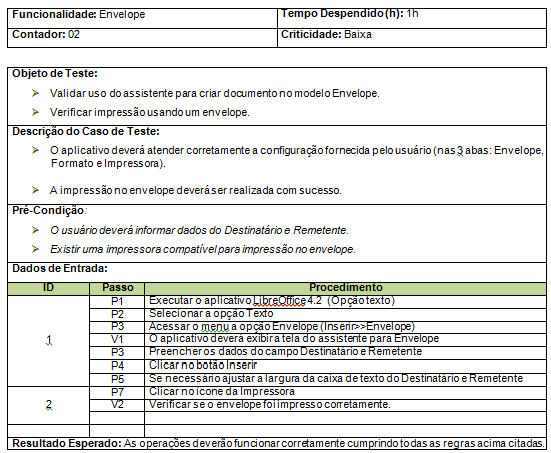
\includegraphics[width=14cm]{img/Capturar.PNG}
\caption{Exemplo}
\end{figure}

\section{Medição e Qualidade de Software}

Apresente aqui o formato da Medição e qualidade de software. Você deve mostrar os meios que irá avaliar a qualidade do seu software. Apresente o plano e os resultados a partir da prática de ferramentas de detecção de code smells, por exemplo.  Em Java, temos uma  ferramenta chamada JDEODORANT.  Você pode avaliar as métricas de qualidade também, por exemplo, em Java, temos CKMetrics\footnote{https://github.com/mauricioaniche/ck}

\section{Observações}

Apresente aqui as dificuldades na disciplina,  trabalho prático e coisas do tipo. 

\newpage
\section{Referências}

[1] Sommerville, Ian -- Software Engineering, 8th Edition;

\end{document}